\section{Agent Modeling with Neural Networks}

% =========================================================
% Motivation: why agent modeling at all?
% =========================================================
\begin{frame}
\frametitle{Why Agent Modeling?}

\centering
{\large\textbf{How do previous MARL methods handle other agents?}}

\vspace{0.75em}

\noindent
\begin{minipage}[c][1.10cm][c]{0.20\textwidth}
    \centering
    \fcolorbox{blue!20}{zhcolor!7}{\parbox[c][0.82cm][c]{2.15cm}{\centering\color{zhcolor}\bfseries\scriptsize Independent\\Learning}}
\end{minipage}\hfill
\begin{minipage}[c][1.10cm][c]{0.39\textwidth}
    \centering
    \small Treat others as part of the environment.
\end{minipage}\hfill
\begin{minipage}[c][1.10cm][c]{0.34\textwidth}
    \raggedright
    {\footnotesize\color{black!55} \textrm{e.g.} opponent behavior affects reward and next state}
\end{minipage}

\vspace{0.25em}
\color{gray!30}\rule{\textwidth}{0.4pt}
\color{black}\vspace{0.25em}

\noindent
\begin{minipage}[c][1.10cm][c]{0.20\textwidth}
    \centering
    \fcolorbox{blue!20}{zhcolor!7}{\parbox[c][0.82cm][c]{2.15cm}{\centering\color{zhcolor}\bfseries\scriptsize Centralized\\Critic}}
\end{minipage}\hfill
\begin{minipage}[c][1.10cm][c]{0.39\textwidth}
    \centering
    \small Uses joint observations/actions during training.
\end{minipage}\hfill
\begin{minipage}[c][1.10cm][c]{0.34\textwidth}
    \raggedright
    {\footnotesize\color{black!55} \textrm{e.g.} COMA critic conditions on the joint action}
\end{minipage}

\vspace{0.25em}
\color{gray!30}\rule{\textwidth}{0.4pt}
\color{black}\vspace{0.25em}

\noindent
\begin{minipage}[c][1.10cm][c]{0.20\textwidth}
    \centering
    \fcolorbox{blue!20}{zhcolor!7}{\parbox[c][0.82cm][c]{2.15cm}{\centering\color{zhcolor}\bfseries\scriptsize Value\\Decomposition}}
\end{minipage}\hfill
\begin{minipage}[c][1.10cm][c]{0.39\textwidth}
    \centering
    \small Uses centralized training information.
\end{minipage}\hfill
\begin{minipage}[c][1.10cm][c]{0.34\textwidth}
    \raggedright
    {\footnotesize\color{black!55} \textrm{e.g.} global state in QMIX}
\end{minipage}

\vspace{0.50em}

{\color{red!70!black}\textbf{\small Still no explicit modeling of other agents' policies}}

\vspace{0.08em}

{\color{green!60!black}\bfseries Agent Modeling:} {\color{black} Learn an explicit model of other agents' policies.}

\end{frame}

% =========================================================
% Slide S2: from tabular JAL-AM to deep JAL-AM
% =========================================================
\subsection{Joint action learning}
\begin{frame}
\frametitle{From Tabular JAL-AM to Deep JAL-AM}

\definecolor{zhcolor}{RGB}{45,88,140}
\centering
\begin{minipage}[t]{0.47\textwidth}
    \centering
    \vspace{-0.75cm}
    \textbf{\small Tabular JAL-AM}\\[0.42em]
    \vspace{-0.10em}
    \fcolorbox{zhcolor!20}{zhcolor!4}{\parbox[c][0.62cm][c]{0.86\linewidth}{\centering\color{zhcolor} State}}\\[0.82em]
    \textbf{Representation}\\[0.72em]
    \fcolorbox{zhcolor!35}{zhcolor!12}{\parbox[c][0.72cm][c]{0.86\linewidth}{\centering\color{zhcolor} Lookup Table}}\\[0.70em]
    \parbox[c][1.42cm][c]{0.86\linewidth}{\centering $A = 8, B = 2$\\[0.22em]$\downarrow$\\[0.20em]$\hat{\pi}(A \mid s)=0.8$\\[0.14em]$\hat{\pi}(B \mid s)=0.2$}\\[0.62em]
    \parbox[c][0.95cm][c]{0.86\linewidth}{\centering\fontsize{15}{16}\selectfont\color{red!70!black} $\times$\\[-0.15em]\large Cannot generalize to unseen states}
\end{minipage}\hfill
\begin{minipage}[t]{0.47\textwidth}
    \centering
    \vspace{-0.75cm}
    \textbf{\small Deep JAL-AM}\\[0.42em]
    \vspace{-0.10em}
    \fcolorbox{zhcolor!20}{zhcolor!4}{\parbox[c][0.62cm][c]{0.86\linewidth}{\centering\color{zhcolor} Observation History}}\\[0.82em]
    \textbf{Representation}\\[0.72em]
    \fcolorbox{zhcolor!35}{zhcolor!12}{\parbox[c][0.72cm][c]{0.86\linewidth}{\centering\color{zhcolor} Neural Network}}\\[0.70em]
    \parbox[c][1.42cm][c]{0.86\linewidth}{\centering Learned mapping\\[0.22em]$\downarrow$\\[0.20em]$\hat{\pi}(A \mid h)=0.8$\\[0.14em]$\hat{\pi}(B \mid h)=0.2$}\\[0.62em]
    \parbox[c][0.95cm][c]{0.86\linewidth}{\centering\fontsize{15}{16}\selectfont\color{green!55!black} $\checkmark$\\[-0.15em]\large Generalizes to unseen observations}
\end{minipage}

\end{frame}

% =========================================================
% Slide S3: deep JAL-AM overview
% =========================================================
\begin{frame}
\frametitle{Deep JAL-AM Overview}

\definecolor{zhcolor}{RGB}{45,88,140}
\centering
{
\small
\textcolor{red!70!black}{\bfseries Challenge:} \tikz[baseline=(de.base)]{\node[
    fill=yellow!15,
    rounded corners=1pt,
    inner xsep=2pt,
    inner ysep=0.4pt
] (de) {Decentralized execution};}
$\rightarrow$ Cannot observe other agents' actions\\[0.20em]
\textcolor{green!55!black}{\bfseries Idea:} Predict other agents' policies
}

\vspace{0.25em}

\resizebox{0.76\textwidth}{!}{%
\begin{tikzpicture}[
    >=Latex,
    every node/.style={font=\small},
    flow/.style={->, thin, draw=gray!60},
    box/.style={
        draw=zhcolor!25,
        fill=zhcolor!4,
        line width=0.45pt,
        minimum width=3.55cm,
        minimum height=0.68cm,
        inner sep=3pt,
        align=center
    },
    modelbox/.style={
        box,
        draw=green!45!black,
        fill=green!13,
        minimum height=0.78cm
    },
    distbox/.style={
        box,
        fill=white,
        minimum width=3.90cm,
        minimum height=1.25cm
    },
    mergebox/.style={
        box,
        draw=zhcolor!35,
        fill=zhcolor!8,
        minimum width=2.95cm,
        minimum height=0.76cm
    },
    actionbox/.style={
        box,
        fill=white,
        minimum width=2.55cm,
        minimum height=0.68cm
    }
]
    % branch titles
    \node[font=\bfseries\small, text=zhcolor] (ltitle) at (-3.9,2.55) {Other agents};
    \node[font=\bfseries\small, text=zhcolor] (rtitle) at (3.9,2.55) {Main agent};

    % left branch
    \node[box] (obsL) at (-3.9,1.72) {Observation History};
    \node[modelbox] (am) at (-3.9,0.78) {Agent Model Network};
    \node[distbox] (dist) at (-3.9,-0.62) {%
        \textcolor{zhcolor}{Predicted Action Distribution}\\[-0.08em]
        \scriptsize Action A : 10\%\\[-0.02em]
        \scriptsize Action B : 70\%\\[-0.02em]
        \scriptsize Action C : 20\%
    };

    % right branch
    \node[box] (obsR) at (3.9,1.72) {Observation History};
    \node[box, fill=zhcolor!7, minimum height=0.78cm] (qnet) at (3.9,0.78) {Q-network};

    % merge
    \node[mergebox] (exp) at (0,-1.98) {Best Response};
    \node[actionbox] (act) at (0,-2.98) {My Action};

    % arrows
    \draw[flow] (obsL) -- (am);
    \draw[flow] (am) -- (dist);
    \draw[flow] (dist.south) -- (exp.north west);
    \draw[flow] (obsR) -- (qnet);
    \draw[flow] (qnet.south) -- (exp.north east);
    \draw[flow] (exp) -- (act);
\end{tikzpicture}%
}

\end{frame}

% =========================================================
% Slide S4: training Deep JAL-AM, agent model + replay buffer
% =========================================================
\begin{frame}
\frametitle{Training Deep JAL-AM}
\framesubtitle{Algorithm Steps 1 \& 2}

\definecolor{zhcolor}{RGB}{45,88,140}

\vspace{-3.60em}
\centering
\begin{tikzpicture}[
    >=Latex,
    every node/.style={font=\small},
    algarrow/.style={->, thin, draw=zhcolor!75},
    block/.style={
        draw=zhcolor!22,
        fill=white,
        line width=0.45pt,
        inner sep=5pt,
        align=center
    },
    smallbox/.style={
        draw=zhcolor!18,
        fill=white,
        line width=0.4pt,
        minimum height=0.36cm,
        inner xsep=5pt,
        inner ysep=2pt,
        align=center
    },
    modelsmall/.style={
        smallbox,
        draw=green!45!black,
        fill=green!13
    },
    num/.style={
        text=red!70!black,
        font=\bfseries\scriptsize,
        inner sep=0pt,
        anchor=east
    }
]

% Left: algorithm image with four static highlights.
\begin{scope}[x=5.62cm,y=6.34cm,yshift=-0.22cm]
    \node[anchor=south west, inner sep=0pt] (algimg) at (0,0) {%
        \IfFileExists{media/deep_jalam_training.png}{%
            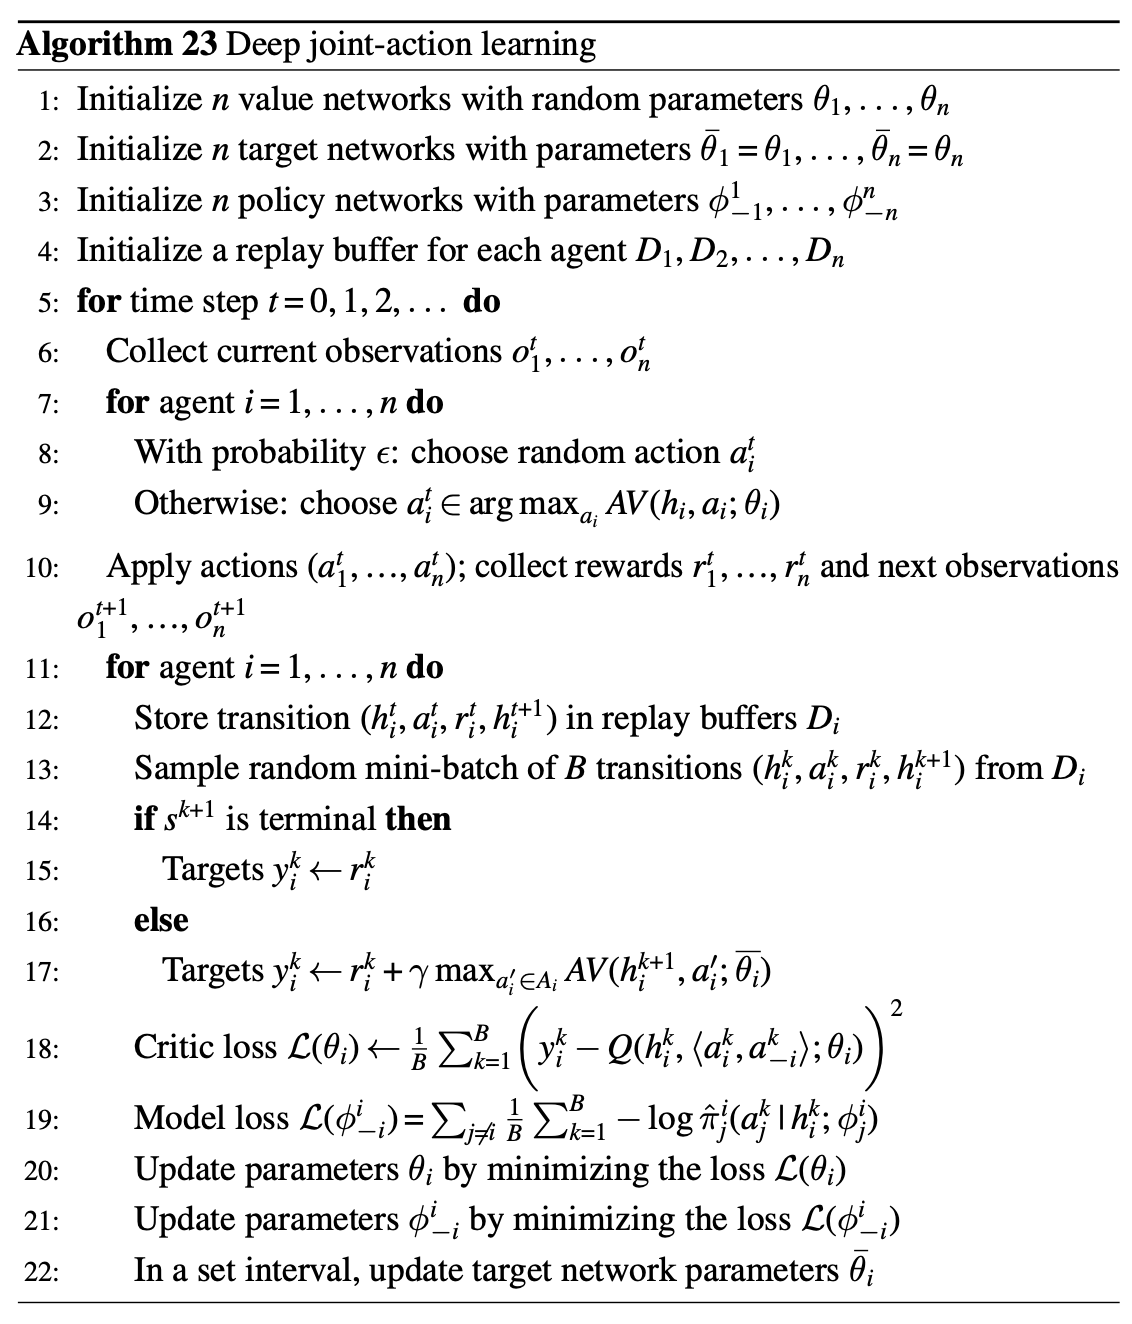
\includegraphics[width=5.62cm,height=6.34cm]{media/deep_jalam_training.png}%
        }{%
            \includegraphics[width=5.62cm,height=6.34cm]{media/deep_jalam_trainig.png}%
        }%
    };

    \fill[yellow!75, opacity=0.40] (0.045,0.842) rectangle (0.900,0.875);
    \fill[yellow!75, opacity=0.40] (0.045,0.797) rectangle (0.890,0.830);
    \fill[yellow!75, opacity=0.40] (0.100,0.188) rectangle (0.940,0.236);
    \fill[yellow!75, opacity=0.40] (0.100,0.142) rectangle (0.940,0.178);

    \node[num] (n1) at (0.036,0.866) {1};
    \node[num] (n2) at (0.036,0.801) {2};
    \node[num] (n4) at (0.088,0.212) {4};
    \node[num] (n3) at (0.088,0.160) {3};

    \coordinate (h1) at (0.905,0.858);
    \coordinate (h2) at (0.895,0.813);
\end{scope}
\draw[gray!35, thin] (0,-0.22) rectangle (5.62,6.12);

% Right: explanations for points 1 and 2.
\node[block, anchor=north west, text width=6.25cm, minimum height=2.52cm] (agentblock) at (6.35,5.95) {%
    \raggedright\textcolor{zhcolor}{\bfseries 1. Agent Model Network}

    \vspace{0.06em}
    \centering
    \scriptsize
    \begingroup
    \setlength{\fboxsep}{1.5pt}
    \fcolorbox{zhcolor!18}{white}{\parbox[c][0.27cm][c]{2.85cm}{\centering Observation history}}\\[-0.18em]
    {\tiny $\downarrow$}\\[-0.18em]
    \fcolorbox{green!45!black}{green!13}{\parbox[c][0.30cm][c]{2.85cm}{\centering Agent model network}}\\[-0.18em]
    {\tiny $\downarrow$}\\[-0.18em]
    \fcolorbox{zhcolor!18}{white}{\parbox[c][0.56cm][c]{3.25cm}{\centering Predicted action distribution\\[-0.12em]
    \tiny A: 10\%\quad B: 70\%\quad C: 20\%}}
    \endgroup

    \vspace{0.08em}
    {\scriptsize Predicts an action distribution \textbf{for each other agent}.}
};

\node[block, anchor=north west, text width=6.25cm, minimum height=2.72cm] (bufferblock) at (6.35,2.82) {%
    \raggedright\textcolor{zhcolor}{\bfseries 2. Replay Buffer}

    \vspace{0.10em}
    \centering
    \small $D_1,\ldots,D_n$\\[-0.08em]
    {\scriptsize Each $D_i$ stores transitions from agent $i$'s perspective:\\[-0.06em]
    $(h_i, a_i, r_i, h'_i)$}

    \vspace{0.28em}
    \begin{tabular}{@{}c@{\hspace{0.35em}$\rightarrow$\hspace{0.35em}}c@{}}
    History $h_i$ & input\\
    Other-agent action \begingroup\setlength{\fboxsep}{0.6pt}\colorbox{red!10}{$a_j$}\endgroup & \textbf{ground-truth label}
    \end{tabular}

    \vspace{0.24em}
    \parbox{5.55cm}{\centering\scriptsize Observed actions from sampled transitions become labels for training the agent model.}
};

% Connect only the explained algorithm points.
\draw[algarrow] (h1) -- (6.09,5.22) -- (6.09,4.70) -- (6.35,4.70);
\draw[algarrow] (h2) -- (6.21,4.93) -- (6.21,1.46) -- (6.35,1.46);
\path[use as bounding box] (0,0) rectangle (12.70,6.34);

\end{tikzpicture}

\end{frame}

% =========================================================
% Slide S5: training objectives, algorithm steps 3 and 4
% =========================================================
\begin{frame}
\frametitle{Training Deep JAL-AM}
\framesubtitle{Algorithm Steps 3 \& 4}

\definecolor{zhcolor}{RGB}{45,88,140}

\vspace{-0.45em}
\centering
\begin{tikzpicture}[
    >=Latex,
    every node/.style={font=\small},
    algarrow/.style={->, thin, draw=zhcolor!75},
    block/.style={
        draw=zhcolor!22,
        fill=white,
        line width=0.45pt,
        inner sep=5pt,
        align=center
    },
    num/.style={
        text=red!70!black,
        font=\bfseries\scriptsize,
        inner sep=0pt,
        anchor=east
    }
]

% Left: algorithm image with the same four static highlights as S4.
\begin{scope}[x=5.62cm,y=6.34cm]
    \node[anchor=south west, inner sep=0pt] (algimg) at (0,0) {%
        \IfFileExists{media/deep_jalam_training.png}{%
            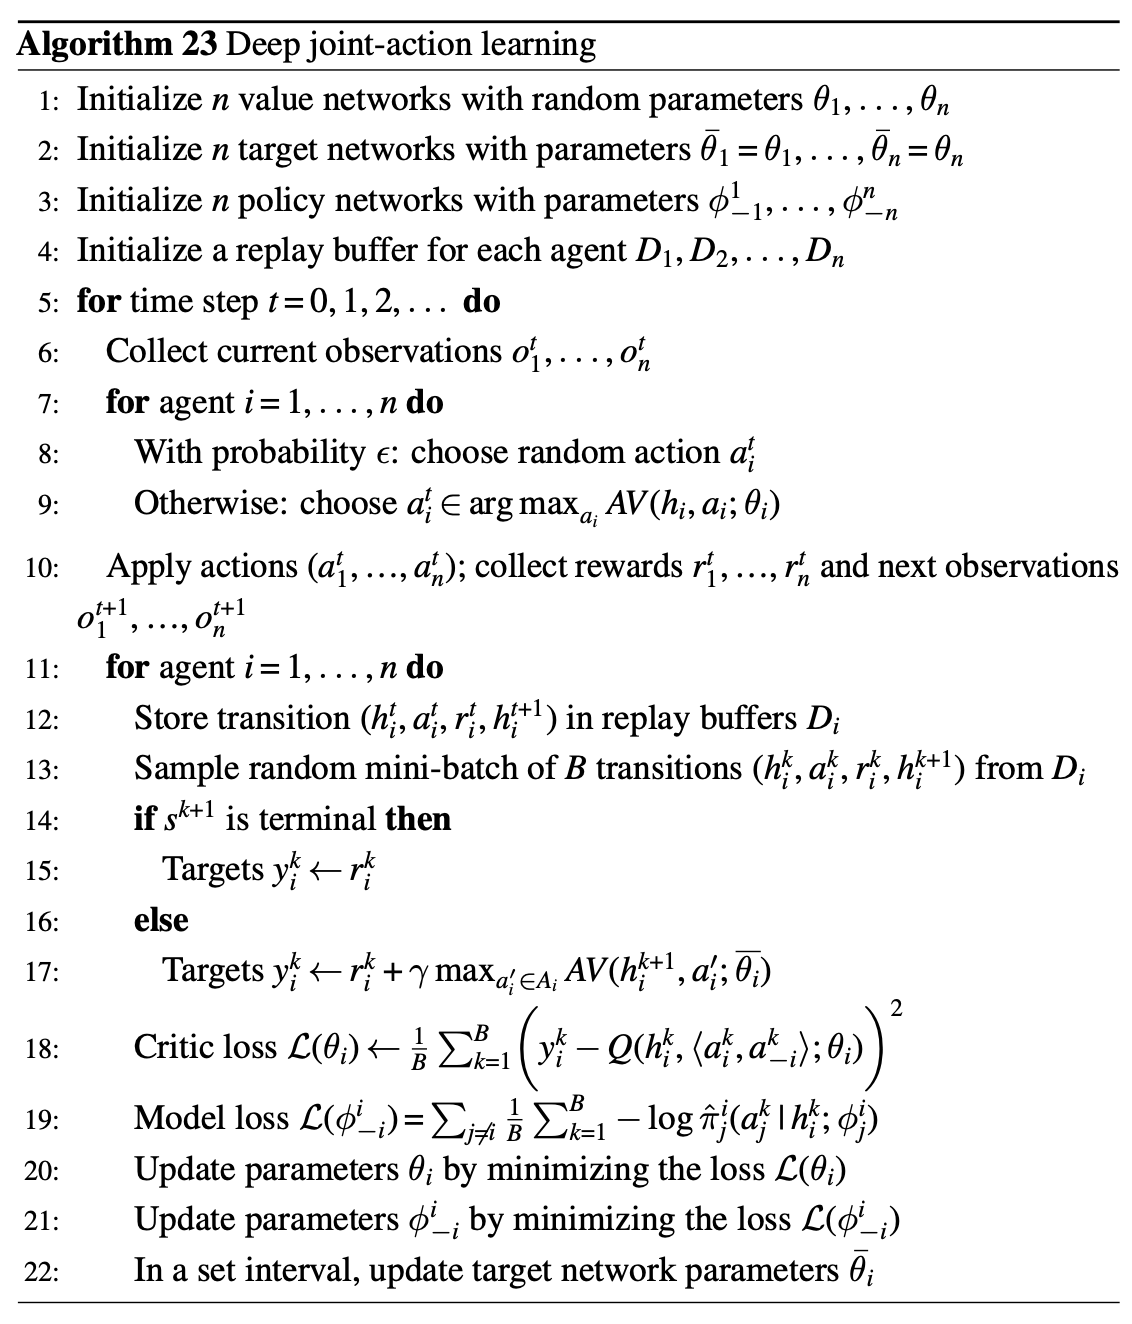
\includegraphics[width=5.62cm,height=6.34cm]{media/deep_jalam_training.png}%
        }{%
            \includegraphics[width=5.62cm,height=6.34cm]{media/deep_jalam_trainig.png}%
        }%
    };

    \fill[yellow!75, opacity=0.40] (0.045,0.842) rectangle (0.900,0.875);
    \fill[yellow!75, opacity=0.40] (0.045,0.797) rectangle (0.890,0.830);
    \fill[yellow!75, opacity=0.40] (0.100,0.188) rectangle (0.940,0.236);
    \fill[yellow!75, opacity=0.40] (0.100,0.142) rectangle (0.940,0.178);

    \node[num] (n1) at (0.036,0.866) {1};
    \node[num] (n2) at (0.036,0.801) {2};
    \node[num] (n4) at (0.088,0.212) {4};
    \node[num] (n3) at (0.088,0.160) {3};

    \coordinate (h4) at (0.945,0.212);
    \coordinate (h3) at (0.945,0.160);
\end{scope}
\draw[gray!35, thin] (0,0) rectangle (5.62,6.34);

% Right: objectives explained for algorithm points 3 and 4.
\draw[draw=zhcolor!22, fill=white, line width=0.45pt] (6.35,6.10) rectangle (12.70,3.38);
\node[anchor=west, font=\bfseries\small, text=zhcolor] at (6.50,5.88) {3. Agent Model Loss};
\node[anchor=center] at (9.55,5.56) {%
    {\scriptsize
    $\displaystyle
    \mathcal{L}(\phi_j^i)
    =
    - \log \hat{\pi}_j^i (
    \begingroup\setlength{\fboxsep}{0.6pt}\colorbox{red!10}{$a_j^t$}\endgroup
    \mid h_i^t; \phi_j^i)
    $}%
};
\node[anchor=center] at (9.55,4.58) {%
    \begingroup
    \setlength{\fboxsep}{1.8pt}
    \begin{tabular}{@{}c@{\hspace{0.36cm}}c@{}}
    \fcolorbox{zhcolor!18}{zhcolor!3}{%
        \parbox[c][1.20cm][c]{1.85cm}{\centering
        {\tiny\bfseries Prediction}\\[0.02em]
        {\tiny A: 0.60}\\[-0.03em]
        {\tiny\textcolor{green!45!black}{\bfseries B: 0.30}}\\[-0.03em]
        {\tiny C: 0.10}}}
    &
    \fcolorbox{zhcolor!18}{zhcolor!3}{%
        \parbox[c][1.20cm][c]{2.35cm}{\centering
        {\tiny\bfseries Ground Truth}\\[0.12em]
        {\tiny Observed action: \textcolor{green!45!black}{\bfseries B}}}}
    \end{tabular}%
    \endgroup
};
\node[anchor=center, font=\tiny] at (9.55,3.60) {Cross-entropy {\color{red}\bfseries penalizes}\ low probability assigned to the observed action.};

\node[block, anchor=north west, text width=6.25cm, minimum height=3.35cm] (valueblock) at (6.35,3.38) {%
    \raggedright\textcolor{zhcolor}{\bfseries 4. Joint-Action Value Function}

    \vspace{0.18em}
    \centering
    \adjustbox{max width=6.00cm}{%
    $\displaystyle
    \mathcal{L}(\theta_i)
    =
    \frac{1}{B}
    \sum_{(h_i^t, a^t, r_i^t, h_i^{t+1}) \in B}
    \left(
    r_i^t
    + \gamma \max_{a_i' \in A_i} \begingroup\setlength{\fboxsep}{0.6pt}\colorbox{red!10}{$AV$}\endgroup(h_i^{t+1}, a_i'; \bar{\theta}_i)
    - Q(h_i^t, \langle a_i^t, a_{-i}^t \rangle; \theta_i)
    \right)^{2}
    $}

    \vspace{0.36em}
    \parbox{5.55cm}{\raggedright\scriptsize
    \textbullet\ DQN-style \textcolor{zhcolor}{\bfseries temporal-difference} objective\\[0.04em]
    \textbullet\ Uses predicted action distributions\\[0.04em]
    \textbullet\ Updates centralized Q-network}
};

% Connect only the objective lines from the algorithm.
\draw[algarrow] (h3) -- (5.90,1.01) -- (5.90,4.85) -- (6.35,4.85);
\draw[algarrow] (h4) -- (6.10,1.34) -- (6.10,1.90) -- (6.35,1.90);

\end{tikzpicture}

\end{frame}

% =========================================================
% Action values with agent models (Eq 9.82, 9.83)
% =========================================================
\begin{frame}
\frametitle{Sampled Action Value}

\definecolor{zhcolor}{RGB}{45,88,140}

\vspace{-0.45em}
\begin{columns}[T,onlytextwidth]

\begin{column}{0.59\textwidth}
\centering
\fcolorbox{zhcolor!25}{zhcolor!6}{\parbox[c][0.30cm][c]{0.84\linewidth}{\centering\color{zhcolor}\bfseries\scriptsize Exact Action Value}}

\vspace{0.06em}
\adjustbox{max width=0.90\linewidth}{%
$\begin{aligned}
AV(h_i, a_i; \theta_i)
&=
\begingroup\setlength{\fboxsep}{0.6pt}\colorbox{zhcolor!10}{$\displaystyle\sum_{a_{-i} \in A_{-i}}$}\endgroup
Q(h_i, \langle a_i, a_{-i} \rangle; \theta_i)\,
\hat{\pi}_{-i}^{i}(a_{-i} \mid h_i; \phi_{-i}^i)
\\[0.4em]
&=
\begingroup\setlength{\fboxsep}{0.6pt}\colorbox{zhcolor!10}{$\displaystyle\sum_{a_{-i} \in A_{-i}}$}\endgroup
Q(h_i, \langle a_i, a_{-i} \rangle; \theta_i)
\prod_{j \ne i}
\hat{\pi}_j^i(a_j \mid h_i; \phi_j^i)
\end{aligned}$}

\vspace{0.02em}
{\scriptsize Uses every possible action combination.}

\vspace{0.06em}
{\scriptsize\bfseries\color{red!70!black} Computationally expensive}

\vspace{0.05em}
{\Large\color{gray!65}$\downarrow$}

\vspace{0.05em}
\fcolorbox{green!45!black}{green!10}{\parbox[c][0.30cm][c]{0.84\linewidth}{\centering\color{green!45!black}\bfseries\scriptsize Sampled Action Value}}

\vspace{0.06em}
\adjustbox{max width=0.90\linewidth}{%
$\begin{aligned}
AV(h_i, a_i; \theta_i)
&=
\frac{1}{\begingroup\setlength{\fboxsep}{0.6pt}\colorbox{zhcolor!10}{$K$}\endgroup}
\sum_{k=1}^{\begingroup\setlength{\fboxsep}{0.6pt}\colorbox{zhcolor!10}{$K$}\endgroup}
Q(h_i, \langle a_i, a_{-i}^k \rangle; \theta_i),
\qquad
a_j^k \sim \hat{\pi}_j^i(\cdot \mid h_i)
\end{aligned}$}

\vspace{0.10em}
{\scriptsize Approximate the expectation\\[-0.05em]using only $K$ sampled joint actions.}
\end{column}

\begin{column}{0.38\textwidth}
\centering
\vspace{0.00em}
\fcolorbox{zhcolor!25}{zhcolor!6}{\parbox[c][0.30cm][c]{0.78\linewidth}{\centering\color{zhcolor}\bfseries\scriptsize Performance Comparison}}

\vspace{0.01em}
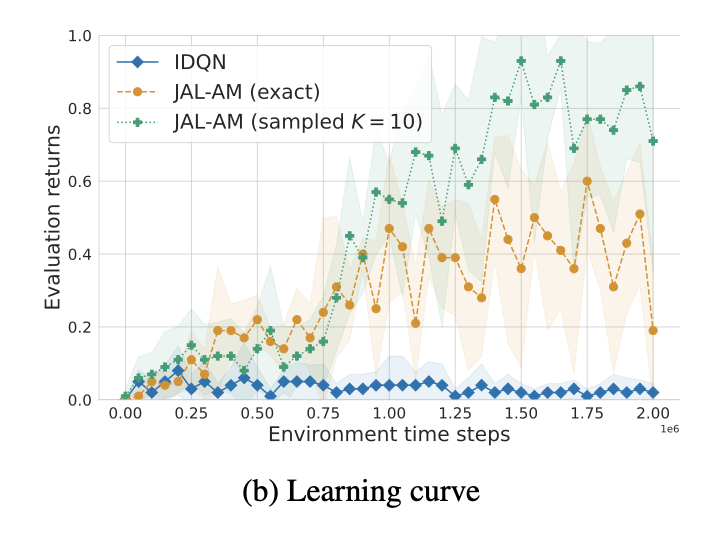
\includegraphics[width=0.84\linewidth,trim={0 42bp 0 0},clip]{media/Sampled vs. exact.png}

\vspace{-0.04em}
\begingroup
\newcommand{\avExampleMathStyle}{\tiny}
\newcommand{\avExampleBody}{\fontsize{6pt}{6.45pt}\selectfont}
\newcommand{\avExampleExplain}{\fontsize{6pt}{6.45pt}\selectfont}
\newcommand{\avExampleHeading}{\fontsize{6.0pt}{6.6pt}\selectfont\bfseries}

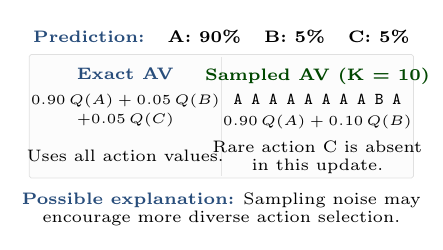
\begin{tikzpicture}[x=1cm,y=1cm]
\path[use as bounding box] (0,0.00) rectangle (4.92,2.46);

\node[anchor=north,inner sep=0pt] at (2.46,2.44)
  {{\avExampleHeading\textcolor{zhcolor!88!black}{Prediction:}\quad
  A: 90\%\quad B: 5\%\quad C: 5\%}};

\draw[draw=gray!24,fill=gray!2,line width=0.24pt,rounded corners=0.7pt] (0.02,0.55) rectangle (4.90,2.12);
\draw[draw=gray!20,line width=0.22pt] (2.46,0.58) -- (2.46,2.09);

\node[anchor=north,inner sep=0pt,text=zhcolor!88!black] at (1.24,1.95)
  {{\avExampleHeading Exact AV}};
\node[anchor=north,inner sep=0pt] at (1.24,1.62)
  {{\avExampleMathStyle\ensuremath{0.90\,Q(A)+0.05\,Q(B)}}};
\node[anchor=north,inner sep=0pt] at (1.24,1.38)
  {{\avExampleMathStyle\ensuremath{+0.05\,Q(C)}}};
\node[anchor=north,inner sep=0pt] at (1.24,0.92)
  {{\avExampleBody Uses all action values.}};

\node[anchor=north,inner sep=0pt,text=green!28!black] at (3.68,1.95)
  {{\avExampleHeading Sampled AV (K = 10)}};
\node[anchor=north,inner sep=0pt] at (3.68,1.62)
  {{\avExampleBody\ttfamily A A A A A A A A B A}};
\node[anchor=north,inner sep=0pt] at (3.68,1.36)
  {{\avExampleMathStyle\ensuremath{0.90\,Q(A)+0.10\,Q(B)}}};
\node[anchor=north,inner sep=0pt] at (3.68,1.03)
  {{\avExampleBody Rare action C is absent}};
\node[anchor=north,inner sep=0pt] at (3.68,0.80)
  {{\avExampleBody in this update.}};

\node[anchor=north,inner sep=0pt] at (2.46,0.37)
  {{\avExampleExplain\textcolor{zhcolor!88!black}{\bfseries Possible explanation:} Sampling noise may}};
\node[anchor=north,inner sep=0pt] at (2.46,0.14)
  {{\avExampleExplain encourage more diverse action selection.}};
\end{tikzpicture}
\endgroup
\end{column}

\end{columns}

\end{frame}

% =========================================================
% Representation learning motivation
% =========================================================
\subsection{Representation Learning}
\begin{frame}
\frametitle{Why Representation Learning?}

\definecolor{zhcolor}{RGB}{45,88,140}
\colorlet{phiBg}{blue!18}
\colorlet{phiBorder}{blue!32!gray}
\newcommand{\phiMinusHighlight}{%
\tikz[baseline=(phih.base)]{
    \node[
        fill=phiBg,
        draw=phiBorder,
        line width=0.14pt,
        rounded corners=1.4pt,
        minimum width=0pt,
        minimum height=0pt,
        inner xsep=2.8pt,
        inner ysep=1.1pt,
        outer sep=0pt,
        font=\scriptsize
    ] (phih) {$\phi_{-i}$};
}}
\colorlet{phiSecondaryBg}{gray!10!blue!4}
\colorlet{phiSecondaryBorder}{gray!22}
\newcommand{\phiMinusSecondary}{%
\tikz[baseline=(phis.base)]{
    \node[
        fill=phiSecondaryBg,
        draw=phiSecondaryBorder,
        line width=0.10pt,
        rounded corners=1.2pt,
        minimum width=0pt,
        minimum height=0pt,
        inner xsep=1.8pt,
        inner ysep=0.7pt,
        outer sep=0pt
    ] (phis) {$\phi_{-i}$};
}}

\vspace{-0.62em}
\centering
\fcolorbox{white}{white}{%
\parbox[c][0.30cm][c]{0.24\linewidth}{\centering
{\color{zhcolor}\bfseries\small Ideal Goal}}}

\vspace{0.06em}
\begin{tikzpicture}[
    box/.style={
        draw=zhcolor!25,
        fill=zhcolor!14,
        line width=0.35pt,
        minimum height=0.44cm,
        align=center,
        inner xsep=4pt,
        inner ysep=1.8pt,
        font=\scriptsize
    },
    sourcebox/.style={
        draw=zhcolor!10,
        fill=zhcolor!1,
        line width=0.25pt,
        minimum height=0.31cm,
        align=center,
        inner sep=0.8pt,
        font=\scriptsize
    },
    arr/.style={-{Stealth[length=2.0mm]}, gray!65, line width=0.45pt}
]
\node[sourcebox, minimum width=2.72cm] (policies)
    {Other agents' policy\\[-0.08em]
            parameters\\[-0.08em]
            {\phiMinusSecondary}};
\node[box, below left=0.46cm and 1.20cm of policies, minimum width=4.10cm] (policy)
    {\textbf{Policy}\\[-0.08em]
    $\pi_i(\cdot \mid h_i,
    \phiMinusHighlight)$};
\node[box, below right=0.46cm and 1.20cm of policies, minimum width=4.10cm] (value)
    {\textbf{Value function}\\[-0.08em]
    $Q_i(h_i, a_i,
    \phiMinusHighlight)$};
\coordinate (split) at ($(policies.south)+(0,-0.18cm)$);
\draw[arr] (policies.south) -- (split);
\draw[arr] (split) -| (policy.north);
\draw[arr] (split) -| (value.north);
\end{tikzpicture}

\vspace{0.04em}
\fcolorbox{zhcolor!18}{zhcolor!4}{%
\parbox[c][0.26cm][c]{0.72\linewidth}{\centering\scriptsize
Condition both the \textbf{policy} and \textbf{value function} on
\textbf{other agents' policies}.}}

\vspace{0.10em}
{\color{gray!45}\rule{0.96\linewidth}{0.35pt}}

\vspace{0.06em}
\fcolorbox{red!25}{red!4}{%
\parbox[c][0.30cm][c]{0.19\linewidth}{\centering
{\color{red!70!black}\bfseries\small Problem}}}

\vspace{0.08em}
\begin{columns}[T,onlytextwidth]
\begin{column}{0.318\textwidth}
\centering
\fcolorbox{gray!35}{gray!5}{%
\begin{minipage}[t][1.94cm][t]{0.90\linewidth}
\centering
{\color{red!70!black}\bfseries\scriptsize Unavailable during decentralized execution}

\vspace{0.08em}
{\scriptsize Other agents' policies cannot be directly observed during
decentralized execution.}
\end{minipage}}
\end{column}

\begin{column}{0.318\textwidth}
\centering
\fcolorbox{gray!35}{gray!5}{%
\begin{minipage}[t][1.94cm][t]{0.90\linewidth}
\centering
{\color{red!70!black}\bfseries\scriptsize Too high-dimensional to condition on}

\vspace{0.16em}
                {\scriptsize $\pi_i(\cdot \mid h_i,
                \phiMinusSecondary)$}

\vspace{0.08em}
\resizebox{0.98\linewidth}{!}{%
{\color{zhcolor}$\phiMinusSecondary =
[\phi_1,\ldots,\phi_{i-1},\phi_{i+1},\ldots,\phi_n]$}}

\vspace{0.08em}
{\scriptsize\color{zhcolor}\bfseries Very large conditioning input}
\end{minipage}}
\end{column}

\begin{column}{0.318\textwidth}
\centering
\fcolorbox{gray!35}{gray!5}{%
\begin{minipage}[t][1.94cm][t]{0.90\linewidth}
\centering
{\color{red!70!black}\bfseries\scriptsize Continuously evolving policies}

\vspace{0.08em}
{\scriptsize Other agents are learning, so their policies are non-stationary.}

\vspace{0.08em}
\resizebox{0.98\linewidth}{!}{%
$\pi_j(a_j \mid h_j; \phi_j^{\,t})
\;\longrightarrow\;
\pi_j(a_j \mid h_j; \phi_j^{\,t+1})$}
\end{minipage}}
\end{column}
\end{columns}

\vspace{0.64em}
\fcolorbox{green!45!black}{green!8}{%
\parbox[c][0.31cm][c]{0.76\linewidth}{\centering\small
Can we learn a {\color{green!45!black}\bfseries compact representation}
instead?}}

\end{frame}

% =========================================================
% Slide S8: encoder-decoder architecture
% =========================================================
\begin{frame}
\frametitle{Encoder--Decoder Architecture}

\definecolor{zhcolor}{RGB}{45,88,140}

\vspace{-0.62em}
\centering
\resizebox{0.96\textwidth}{!}{%
\begin{tikzpicture}[
    >=Latex,
    every node/.style={font=\small},
    flow/.style={->, line width=0.62pt, draw=black!78},
    branch/.style={line width=0.62pt, draw=black!78},
    activeflow/.style={->, line width=0.95pt, draw=green!45!black},
    activebranch/.style={line width=0.95pt, draw=green!45!black},
    fadedflow/.style={->, line width=0.56pt, draw=black!24},
    box/.style={
        rounded corners=4pt,
        line width=0.70pt,
        minimum height=0.88cm,
        inner xsep=8pt,
        inner ysep=5pt,
        align=center
    },
    encoder/.style={
        box,
        draw=orange!70!black,
        fill=orange!15,
        minimum width=2.35cm
    },
    decoder/.style={
        box,
        draw=zhcolor!55,
        fill=zhcolor!10,
        minimum width=2.35cm
    },
    policybox/.style={
        box,
        draw=green!48!black,
        fill=green!12,
        minimum width=3.50cm
    },
    repr/.style={
        draw=red!65!black,
        fill=white,
        line width=0.92pt,
        rounded corners=2pt,
        inner xsep=4pt,
        inner ysep=2pt,
        align=center
    },
    status/.style={
        anchor=west,
        align=left,
        font=\scriptsize
    },
    modulelabel/.style={
        font=\footnotesize\bfseries,
        text=black!86,
        align=center
    },
    modulelabelinactive/.style={
        modulelabel,
        text=black!42
    },
    mathnode/.style={font=\large}
]
\path[use as bounding box] (-0.55,-1.05) rectangle (10.75,2.72);

\only<1>{%
\node[mathnode] (hist) at (0,0) {$h_i^t$};
\node[encoder] (enc) at (2.00,0) {$f^e(h_i^t; \psi_i^e)$};
\node[repr] (rep) at (3.95,0) {$m_i^t$};
\node[decoder] (dec) at (6.00,0) {$f^d(m_i^t; \psi_i^d)$};
\node[mathnode] (pihat) at (8.10,0) {$\hat{\pi}_{-i}^{\,i,t}$};
\node[policybox] (policy) at (6.35,1.58)
    {$\pi(\cdot \mid h_i^t, m_i^t; \phi_i)$};
\node[mathnode] (action) at (9.45,1.58) {$a_i^t$};
\node[modulelabel, above=0.02cm of enc] {Encoder};
\node[modulelabel, above=0.02cm of policy] {Policy};
\node[modulelabel, above=0.02cm of dec] {Decoder};

\draw[flow] (hist.east) -- (enc.west);
\draw[flow] (enc.east) -- (rep.west);
\draw[flow] (rep.east) -- (dec.west);
\draw[flow] (dec.east) -- (pihat.west);
\draw[flow] (policy.east) -- (action.west);
\draw[branch] (hist.north) -- (0,1.58) -- (4.35,1.58);
\draw[branch] (rep.north) -- (3.95,1.58);
\draw[flow] (4.35,1.58) -- (policy.west);

\node[font=\scriptsize\bfseries, text=red!60!black, below=0.12cm of rep]
    {Compact Representation};
\node[status, text=zhcolor] at (-1.02,2.42)
    {{\small\bfseries Training}\\[0.02em]Encoder and Decoder are optimized together.};
}

\only<2>{%
\node[mathnode] (hist) at (0,0) {$h_i^t$};
\node[encoder, draw=green!50!black, line width=0.90pt] (enc) at (2.00,0)
    {$f^e(h_i^t; \psi_i^e)$};
\node[repr, fill=green!7] (rep) at (3.95,0) {$m_i^t$};
\node[decoder, draw=black!18, fill=black!4, text=black!34] (dec) at (6.00,0)
    {$f^d(m_i^t; \psi_i^d)$};
\node[mathnode, text=black!32] (pihat) at (8.10,0) {$\hat{\pi}_{-i}^{\,i,t}$};
\node[policybox, draw=green!50!black, line width=0.90pt] (policy) at (6.35,1.58)
    {$\pi(\cdot \mid h_i^t, m_i^t; \phi_i)$};
\node[mathnode] (action) at (9.45,1.58) {$a_i^t$};
\node[modulelabel, above=0.02cm of enc] {Encoder};
\node[modulelabel, above=0.02cm of policy] {Policy};
\node[modulelabelinactive, above=0.02cm of dec] {Decoder};

\draw[activeflow] (hist.east) -- (enc.west);
\draw[activeflow] (enc.east) -- (rep.west);
\draw[fadedflow] (rep.east) -- (dec.west);
\draw[fadedflow] (dec.east) -- (pihat.west);
\draw[activeflow] (policy.east) -- (action.west);
\draw[activebranch] (hist.north) -- (0,1.58) -- (4.35,1.58);
\draw[activebranch] (rep.north) -- (3.95,1.58);
\draw[activeflow] (4.35,1.58) -- (policy.west);

\node[font=\scriptsize\bfseries, text=red!60!black, below=0.12cm of rep]
    {Compact Representation};
\node[status, text=green!45!black] at (-1.02,2.42)
    {{\small\bfseries Execution}\\[0.02em]Decoder not required for action selection.};
}
\end{tikzpicture}%
}

\vspace{0.34em}
\begin{columns}[T,onlytextwidth]
\begin{column}{0.47\textwidth}
\centering
\fcolorbox{zhcolor!22}{white}{%
\begin{minipage}[t][1.16cm][t]{0.90\linewidth}
{\color{zhcolor}\bfseries\small Encoder}

\vspace{0.07em}
{\footnotesize
\textbullet\ Compresses the observation history\\[0.02em]
\textbullet\ Learns the compact embedding $m_i^t$}
\end{minipage}}
\end{column}

\begin{column}{0.47\textwidth}
\centering
\fcolorbox{zhcolor!22}{white}{%
\begin{minipage}[t][1.16cm][t]{0.90\linewidth}
{\color{zhcolor}\bfseries\small Decoder}

\vspace{0.07em}
{\footnotesize
\textbullet\ Reconstructs other agents' policy distributions\\[0.02em]
\textbullet\ Provides the reconstruction training signal}
\end{minipage}}
\end{column}
\end{columns}

\end{frame}

% =========================================================
% Slide S9: representation learning in A2C
% =========================================================
\begin{frame}
\frametitle{Applying Representation Learning to A2C}

\definecolor{zhcolor}{RGB}{45,88,140}
\newcommand{\mihighlight}{%
\tikz[baseline=(mi.base)]{%
    \node[
        draw=black!35,
        fill=black!16,
        line width=0.22pt,
        rounded corners=1.5pt,
        inner xsep=3.0pt,
        inner ysep=1.0pt
    ] (mi) {$\mathbf{m}_i$};%
}}

\vspace{-0.65em}
\begin{columns}[T,onlytextwidth]
\begin{column}{0.43\textwidth}
\fcolorbox{zhcolor!18}{white}{%
\begin{minipage}[t][2.05cm][t]{0.94\linewidth}
\vspace{0.02em}
{\color{zhcolor}\bfseries\small Representation-based approach}

\vspace{0.12em}
{\centering
{\small Representation-based approach}\\[0.03em]
{\color{gray!65}\normalsize $\downarrow$}\\[0.06em]
{\setlength{\fboxsep}{1.6pt}%
\fcolorbox{orange!30}{orange!10}{%
\parbox[c][0.24cm][c]{0.53\linewidth}{\centering\small\bfseries General framework}}}\par}
\end{minipage}}
\end{column}

\begin{column}{0.54\textwidth}
\fcolorbox{zhcolor!18}{zhcolor!3}{%
\begin{minipage}[t][2.05cm][t]{0.94\linewidth}
\vspace{0.04em}
{\color{zhcolor}\bfseries\small A2C + Agent Modeling}

\vspace{0.22em}
{\small
\textbf{Policy:}\quad
$\pi(\cdot \mid h_i, \mihighlight; \phi_i)$\\[0.16em]
\textbf{Value function:}\quad
$V(h_i, z, \mihighlight; \theta_i)$}

\vspace{0.14em}
{\footnotesize
Both the actor and critic use the learned agent representation,\\[-0.02em]
without modifying the overall A2C framework.}
\end{minipage}}
\end{column}
\end{columns}

\vspace{0.10em}
{\color{gray!45}\rule{\linewidth}{0.35pt}}

\vspace{1.05em}
\hspace*{-0.115\textwidth}%
\begin{minipage}{1.115\textwidth}
\begin{columns}[T,onlytextwidth]
\begin{column}{0.51\textwidth}
\makebox[\linewidth][c]{\hspace*{0.15\linewidth}{\color{zhcolor}\bfseries\small Experimental Result}}

\vspace{0.08em}
\makebox[\linewidth][c]{\hspace*{0.15\linewidth}\fcolorbox{black!18}{white}{%
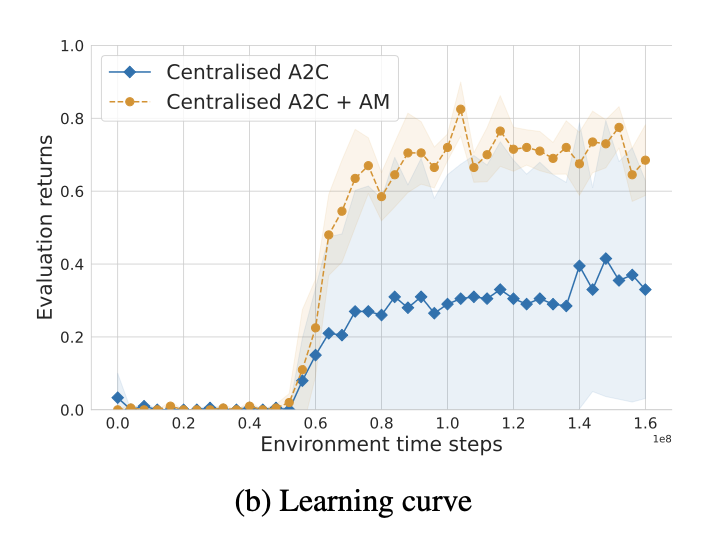
\includegraphics[width=0.98\linewidth,height=3.36cm,keepaspectratio]{media/A2C+AM.png}}}
\end{column}

\begin{column}{0.47\textwidth}
\vspace{1.02em}
\hspace*{-0.04\linewidth}{\setlength{\fboxsep}{4pt}%
\fcolorbox{green!35!black}{green!5}{%
\begin{minipage}[t][3.20cm][t]{0.96\linewidth}
{\color{green!45!black}\bfseries\small With Agent Modeling}

\vspace{0.42em}
{\small
\textbullet\ Learns faster\\[0.28em]
\textbullet\ Higher final return\\[0.28em]
\textbullet\ More consistent learning\\[-0.02em]
\hspace*{0.86em}{{\fontsize{7.8}{9.0}\selectfont Lower variance across runs.}}}
\end{minipage}}}
\end{column}
\end{columns}
\end{minipage}

\end{frame}

% =========================================================
% Slide S10: advanced agent modeling
% =========================================================
\definecolor{zhcolor}{RGB}{45,88,140}

\begin{frame}
\frametitle{Advanced Agent Modeling}

\vspace{-0.56em}
\begin{center}
{\color{black!78}\bfseries\fontsize{11}{12.5}\selectfont Beyond behavior prediction}
\end{center}

\vspace{0.12em}
\begin{columns}[T,onlytextwidth]
\begin{column}{0.49\textwidth}
\fcolorbox{zhcolor!20}{zhcolor!3}{%
\begin{minipage}[t][4.60cm][t]{0.94\linewidth}
\vspace{0.05em}
{\color{zhcolor}\bfseries\small 1. Probabilistic Recursive Reasoning}

\vspace{0.14em}
\centering
{\bfseries\small How will the other agent react?}

\vspace{0.16em}
{\setlength{\fboxsep}{2pt}%
\fcolorbox{zhcolor!25}{zhcolor!6}{%
\parbox{0.88\linewidth}{\centering
{\footnotesize
\textbf{Level 0}\\[-0.05em]
What will B do?\\[-0.02em]
{\color{gray!65}$\downarrow$}\\[-0.03em]
\textbf{Level 1}\\[-0.05em]
What does B believe I will do?\\[-0.02em]
{\color{gray!65}$\downarrow$}\\[-0.03em]
\textbf{Level 2}\\[-0.05em]
What do I believe B believes I will do?}}}}

\vspace{0.34em}
{\scriptsize
Models \textbf{nested beliefs} and \textbf{uncertainty}.}

\vspace{0.36em}
{\footnotesize
{\color{zhcolor}\bfseries Prior}
{\color{gray!60}$\rightarrow$}
Observation
{\color{gray!60}$\rightarrow$}
{\color{zhcolor}\bfseries Posterior}}
\vspace{0.10em}
\end{minipage}}
\end{column}

\begin{column}{0.49\textwidth}
\fcolorbox{orange!35!black!30}{orange!4}{%
\begin{minipage}[t][4.60cm][t]{0.94\linewidth}
\vspace{0.05em}
{\color{orange!65!black}\bfseries\small 2. Opponent Shaping}

\vspace{0.14em}
\centering
{\bfseries\small How will my action influence\\[-0.02em]
their future learning?}

\vspace{0.12em}
{\setlength{\fboxsep}{2pt}%
\fcolorbox{orange!55!black!30}{orange!7}{%
\parbox{0.88\linewidth}{\centering
{\scriptsize
My action\\[-0.07em]
{\color{gray!65}$\downarrow$}\\[-0.09em]
B receives reward\\[-0.07em]
{\color{gray!65}$\downarrow$}\\[-0.09em]
{\setlength{\fboxsep}{1.2pt}\colorbox{orange!14}{\textbf{B} updates its policy}}\\[-0.07em]
{\color{gray!65}$\downarrow$}\\[-0.09em]
{\bfseries B's future behavior changes}\\[-0.07em]
{\color{gray!65}$\downarrow$}\\[-0.09em]
{\bfseries My future return is affected}}}}}

\vfill
{\scriptsize
Choose actions while accounting for\\[-0.05em]
\textbf{how the other agent may learn.}}
\vspace{0.12em}
\end{minipage}}
\end{column}
\end{columns}

\vspace{0.08em}
\begin{center}
{\setlength{\fboxsep}{4.2pt}%
\fcolorbox{black!15}{white}{%
\parbox{0.96\linewidth}{%
\begin{minipage}[t]{0.48\linewidth}
\centering
{\footnotesize
\textbf{Recursive reasoning:}\\[-0.02em]
{\color{zhcolor}\bfseries Predict} how others will react.}
\end{minipage}\hfill
\begin{minipage}[t]{0.48\linewidth}
\centering
{\footnotesize
\textbf{Opponent shaping:}\\[-0.02em]
{\color{orange!75!black}\bfseries Influence} how others will learn.}
\end{minipage}}}}
\end{center}

\end{frame}

% =========================================================
% Final summary
% =========================================================
\begin{frame}
\frametitle{Agent Modeling: Key Takeaways}

\vspace{-0.45em}
\begin{center}
\begin{tikzpicture}[
    >=Latex,
    stage/.style={
        rounded corners=2pt,
        minimum width=4.75cm,
        minimum height=1.78cm,
        text width=4.32cm,
        align=center,
        inner xsep=8pt,
        inner ysep=5pt,
        line width=0.35pt
    },
    flowarrow/.style={->, line width=0.65pt, draw=gray!68, shorten <=2.5pt, shorten >=2.5pt}
]

\node[
    stage,
    draw=black!18,
    fill=zhcolor!2
] (s1) at (0,0) {
    {\color{zhcolor!85}\rule{2.05cm}{0.55pt}}\\[0.26em]
    {\color{zhcolor}\large\bfseries Agent Modeling}\\[0.28em]
    {\scriptsize
    Model other agents explicitly.}
};

\node[
    stage,
    draw=black!18,
    fill=cyan!2
] (s2) at (6.05,0) {
    {\color{cyan!42!black}\rule{2.05cm}{0.55pt}}\\[0.26em]
    {\color{cyan!42!black}\large\bfseries Deep JAL-AM}\\[0.28em]
    {\scriptsize
    Generalize beyond\\
    tabular representations.}
};

\node[
    stage,
    draw=black!18,
    fill=green!2
] (s3) at (0,-2.50) {
    {\color{green!36!black}\rule{2.05cm}{0.55pt}}\\[0.26em]
    {\color{green!36!black}\large\bfseries Representation Learning}\\[0.28em]
    {\scriptsize
    Replace explicit policies\\
    with compact agent embeddings.}
};

\node[
    stage,
    draw=black!18,
    fill=orange!3
] (s4) at (6.05,-2.50) {
    {\color{orange!62!black}\rule{2.05cm}{0.55pt}}\\[0.26em]
    {\color{orange!62!black}\large\bfseries Advanced Agent Modeling}\\[0.28em]
    {\scriptsize
    Predict how others react\\
    and how they may learn.}
};

\draw[flowarrow] (s1.east) -- (s2.west);
\draw[flowarrow] (s2.south west) -- (s3.north east);
\draw[flowarrow] (s3.east) -- (s4.west);

\end{tikzpicture}
\end{center}

\vspace{0.34em}
\begin{center}
{\color{black!20}\rule{0.78\linewidth}{0.4pt}}

\vspace{0.30em}
{\small
Explicit models of other agents enable
{\color{zhcolor}\fontseries{bx}\selectfont better decision-making}
in multiagent environments.}
\end{center}

\end{frame}
